\chapter{CONCLUSION}

Cette étude a permis d’explorer le potentiel des réseaux neuronaux à convolution appliqués filtrage des images QuadPol en milieu urbain. Nous avons implémenté une architecture simple et modulaire nommée \textbf{VDPolSARF} inspirée des réseaux \textbf{VDSR} et \textbf{RESNET}.  Cette architecture nous a permis d'explorer l'effet de différents paramètres dont la taille de la convolution d'entrée, le nombre de convolutions par couche et le nombre de couches du réseaux. Comparées aux approches classiques, les architectures testées ont démontré que les approches en apprentissages machine profond permettent d'obtenir une bonne estimation des paramètres polarimétriques tout en préservant la résolution spatiale aussi bien sinon mieux que ces dernières. De plus, les travaux ont montré qu'il n'est pas nécessaire d'avoir des réseaux extrêmement profonds (5 couches suffises) pour réaliser un bon filtrage. Cependant, certains aspects de ces filtres restent à explorer et à améliorer.

Du point de vue de l'apprentissage, nous pourrions visiter l'espace des paramètres qui sont demeurés fixes durant nos expérimentations afin d'optimiser celui-ci. En particulier, il serait intéressant de vérifier l'impact du paramètre du taux d'apprentissage plus adéquatement sur la vitesse de convergence et la précision. Nous pourrions de plus utiliser des fonctions de coût basées sur des métriques mieux adaptées à la polarimétrie, comme par exemple la distance de Frobenius. Un autre aspect à améliorer serait le balancement des classes polarimétriques, car selon la distribution de nos échantillons sur le plan {\halphans} (Fig. \ref{fig:distribution_halpha_sigs}), certaines de nos classes sont mieux représentées.  L'idéal serait de faire un apprentissage balancé uniformément et vérifier si ceci apporterait de meilleurs résultats.  Toujours en lien avec la distribution des échantillons, nous remarquons qu'ils ne sont pas uniformément répartis sur le plan $H/A$ (Fig. \ref{fig:distribution_ha_sigs} ).  Ce qui nous amène à réfléchir que la production des signatures devrait être distribuée uniformément selon les trois axes {\haalphans} afin qu'il n'y ait pas de biais introduit par rapport à la distribution des valeurs propres des matrices de cohérence.
 
Un problème en lien avec la grande différence des statistiques entre les termes co-polaires et les termes croisés des matrices de cohérence bruitées est que les réseaux se voient obliger de modéliser deux ensembles de données complètement différents.  Nous pourrions réfléchir à une approche où chaque terme de type co-polaire et croisé serait filtré par leur propre réseau. Ceci nous rapproche de la proposition de Lopèz-Martinez et Fàbregas \cite{Lopez2003} qui modéliserait les termes croisés indépendamment des termes copolaires.  La Figure \ref{fig:bi-vdpolsar} présente une architecture qui pourrait aider à résoudre le problème. Elle  est une simple extension de notre meilleur réseau actuel. Ce nouveau réseau serait découpé en deux branches, chaque branche modélise indépendamment un estimateur des paramètres copolaires et un estimateur des paramètres croisés.  En sortie du réseau les estimations sont réordonnées correctement pour former l'estimation complète de la matrice de cohérence.
 
 \begin{figure}
  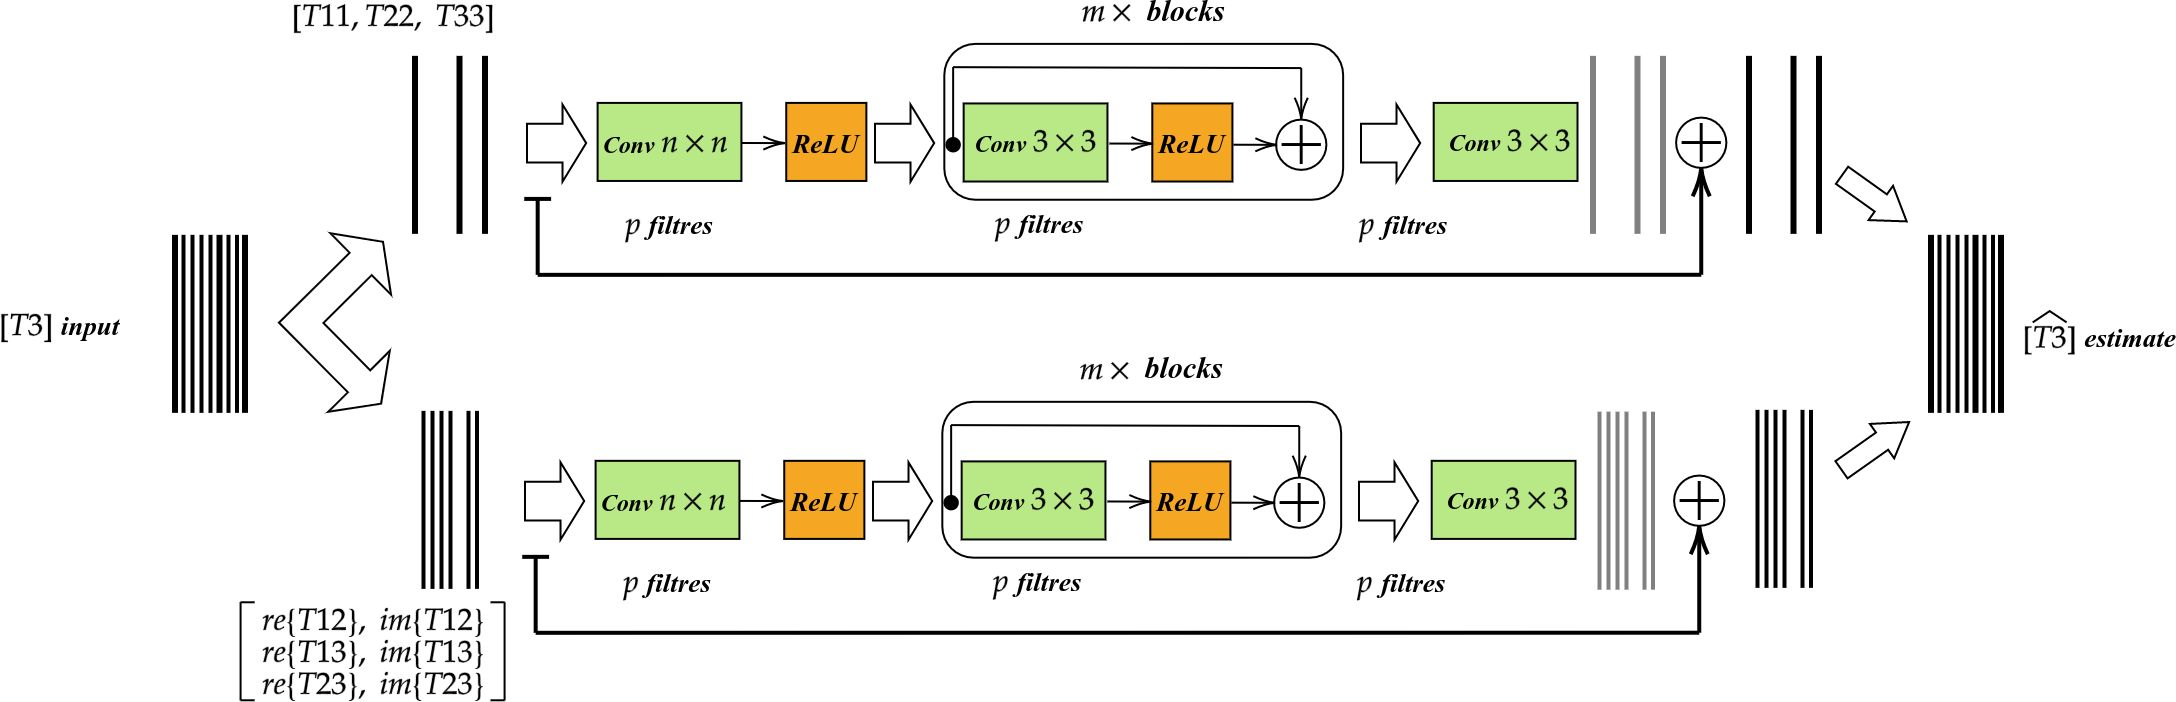
\includegraphics[width=1.0\linewidth]{figures/Conclusion/diagram-20191202.jpg}
  \centering
  \caption{
  \footnotesize{Exemple d'une architecture permettant de filtrer indépendamment les termes copolaires et les termes croisés de la matrice de cohérence. La branche du haut modélise les 3 termes copolaires et la branche du bas modélise chacune des parties des nombres complexes des termes croisés.}
  }
  \label{fig:bi-vdpolsar}
\end{figure}

Pour conclure ce mémoire nous présentons un résultat qualitatif préliminaire de ce réseau bi-céphale.  La Figure \ref{fig:res-bi-vdpolsar} compare nos deux modèles \textbf{VDPolSARF}  présentés auparavant avec le nouveau modèle que nous appellerons \textbf{VDPolSARF-Bi} .  Ce dernier a été entraîné sur les données hétérogènes avec inclusion de cibles ponctuelles. La même méthodologie a été utilisée pour l'entraînement à la différence près que la puissance des cibles ponctuelles a été légèrement augmentée.  La sous-figure en-bas à droite présente notre nouveau résultat qui se compare favorablement aux résultats précédents.  On y remarque que les artéfacts autour des cibles ont disparu et que les zones homogènes semblent bien filtrées.  Les contours et les arêtes semblent bien préservés aussi.  Ce qui nous ouvrent d'autres voies à la recherche qui paraissent valoir la peine d'être explorées.  Mais pour l'instant, nous concluons cette étape des travaux ici.

 \begin{figure}
  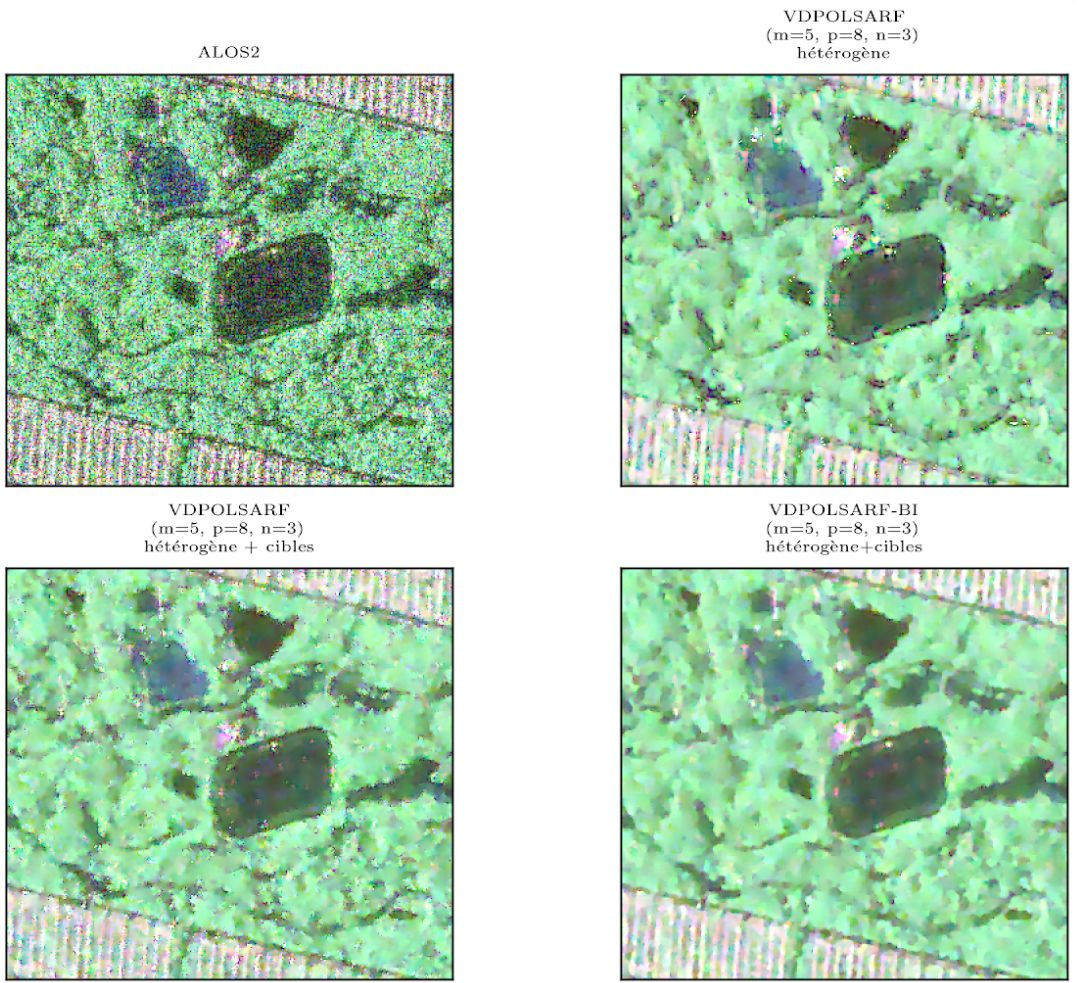
\includegraphics[width=1.0\linewidth]{figures/Conclusion/bi-vspolsar.jpg}
  \centering
  \caption{
  \small{Résultats comparatifs en les modèles antécédents et le résultat de la nouvelle architecture.  En-haut à gauche, l'image ALOS2 une vue. En-haut à droite, le résultat du modèle \textbf{VDPolSARF} entraîné sur les données hétérogènes. En-bas à gauche, le résultat du modèle \textbf{VDPolSARF} entraîné sur les données hétérogènes avec inclusion de cibles ponctuelles.  Et finalement, en-bas à droite, le résulat du modèle bi-céphale \textbf{VDPolSARF-Bi} entraîné sur les données hétérogènes avec inclusion de cibles ponctuelles. $\paulicomposition$ }
  }
  \label{fig:res-bi-vdpolsar}
\end{figure}
